\chapter{Forest for the Trees}
\lettrine[lines=4]{T}{rees} are another special kind of graph which we did not discuss in the previous chapter. Trees are somewhat unique compared to the other types of specialty graphs described before as they allow us certain algorithms to perform to solve different problems. Before we go in depth into trees, we must first define an operation and some other terms.

\section{Definitions}
Let $G_1$ and $G_2$ be graphs. Then $G_1 \cup G_2$ is the \textbf{union} of $G_1$ and $G_2$ with the vertex set $V = V(G_1) \cup V(G_2)$ and edge set $E = E(G_1) \cup E(G_2)$. Now, let's establish some more definitions:
\begin{description}
    \item[Disconnected:] A graph is \textbf{disconnected} if it is the union of two graphs. Here is an example of a disconnected graph:
    \begin{center}
        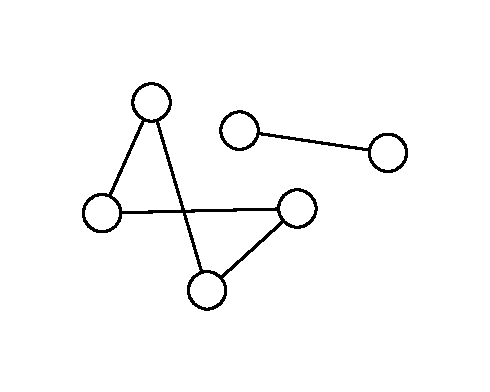
\includegraphics[width=0.3\textwidth]{Chapter2/disconnect.pdf}
    \end{center}
    \item[Connected:] A graph is \textbf{connected} if it is not disconnected (wow). Here is an example of a connected graph:
    \begin{center}
        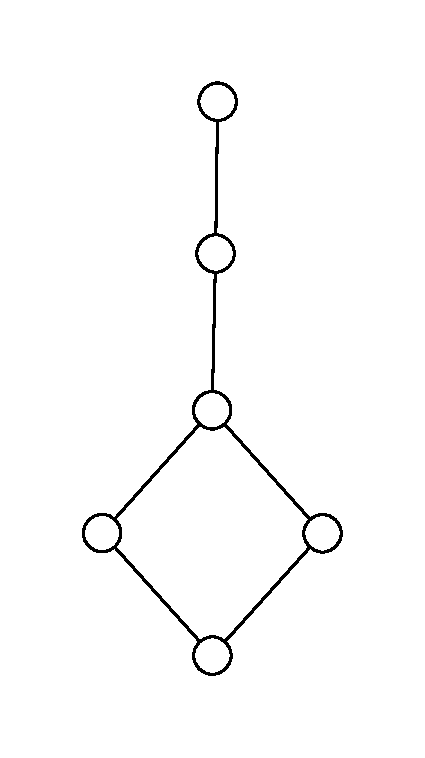
\includegraphics[width=0.3\textwidth]{Chapter2/connect.pdf}
    \end{center}
    \item[Component:] A \textbf{component} graph is one graph which makes up part of a union. In $G = G_1 \cup G_2$, $G_1$ and $G_2$ are components.
\end{description}

We can also define the \textbf{subtraction} of a set of edges $F$ from a graph $G$. We say that $G - F$ is the graph resulting in the removal of the edges in $F$ from $G$. Suppose we have the following graph $G$:
\begin{center}
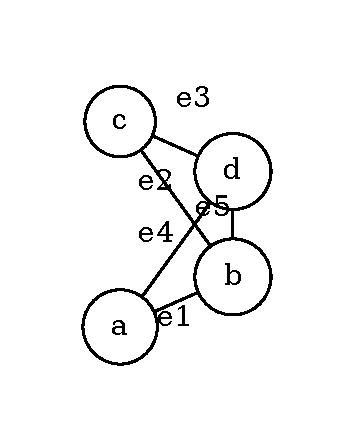
\includegraphics[width=0.3\textwidth]{Chapter2/sub0.pdf}
\end{center}
Then the following are different subtractions from $G$.
\begin{figure}[h]
    \subfloat[$G - \{e1\}$]{
        \begin{minipage}[c][1\width]{0.3\textwidth}
            \centering
            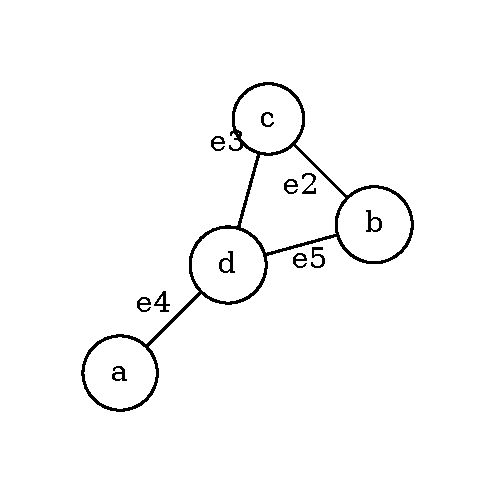
\includegraphics[width=1.\textwidth]{Chapter2/sub1.pdf}
        \end{minipage}
    }
    \subfloat[$G - \{e2\}$]{
        \begin{minipage}[c][1\width]{0.3\textwidth}
            \centering
            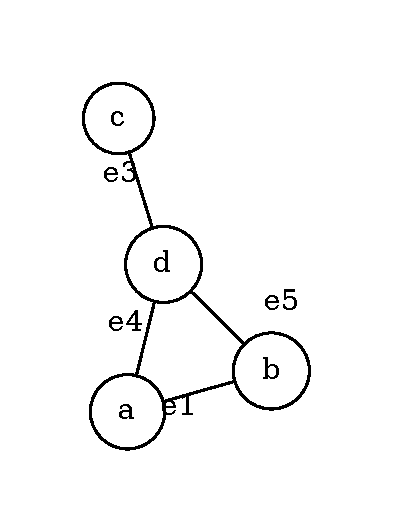
\includegraphics[width=\textwidth]{Chapter2/sub2.pdf}
        \end{minipage}
    }
    \subfloat[$G - \{e1, e2\}$]{
        \begin{minipage}[c][1\width]{0.3\textwidth}
            \centering
            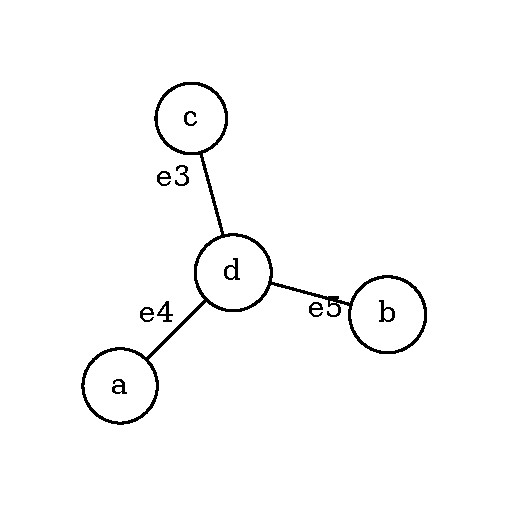
\includegraphics[width=\textwidth]{Chapter2/sub12.pdf}
        \end{minipage}
    }
\end{figure} 

Let's define a new type of graph. A connected graph that is regular of degree 2 is called a \textbf{cycle}, which we denote $C_n$. Here is an example of a cycle, $C_5$:
\begin{center}
    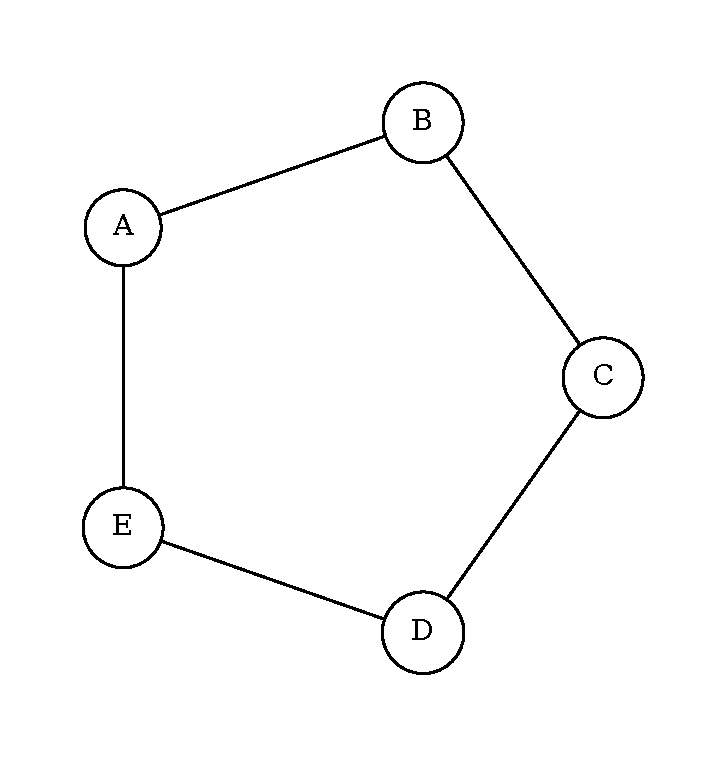
\includegraphics[width=0.3\textwidth]{Chapter2/c5.pdf}
\end{center}

A useful operation on graphs is to take the complement. The \textbf{complement} of a graph $G$ is the graph $\overline{G}$, with vertex set $V(\overline{G}) = V(G)$, with two vertices adjacent in $\overline{G}$ if and only if they are \emph{not} adjacent in $G$. Given $C_5$, we can fine its complement, $\overline{C_5}$:
\begin{center}
    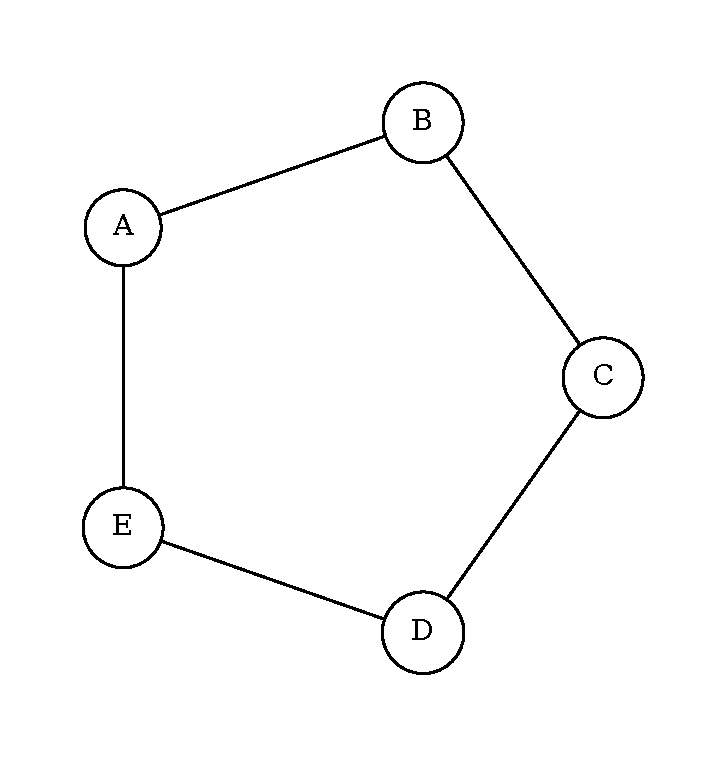
\includegraphics[width=0.3\textwidth]{Chapter2/c5.pdf}
    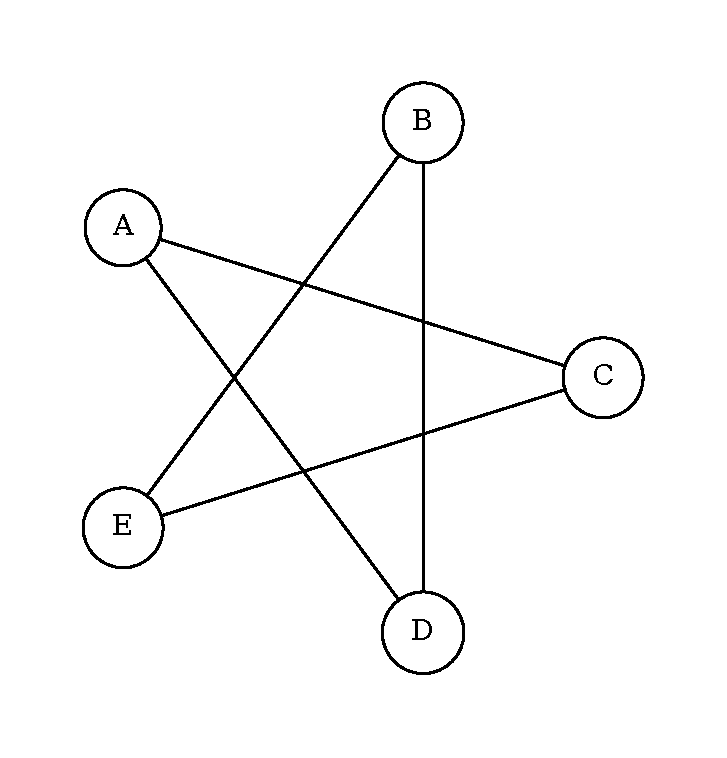
\includegraphics[width=0.3\textwidth]{Chapter2/c5comp.pdf}
\end{center}
In this particular example, notice that $C_5 \sim \overline{C_5}$, so $C_5$ is what we call \textbf{self-complementary} - it is isomorphic to its own complement.

\section{Trailblazing}
We've defined what graphs are as a construct, but how do we actually navigate from one point to another? There are different ways to navigate from vertex to vertex, and each form of navigation takes on different attributes. Consider the following graph $G_0$:
\begin{center}
    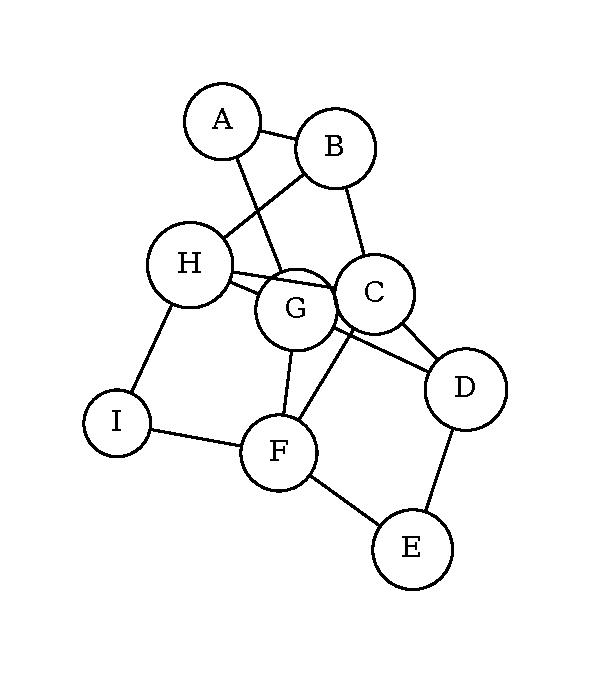
\includegraphics[width=0.5\textwidth]{Chapter2/nav.pdf}
\end{center}
Let's define some of the different ways we can navigate through $G_0$:
\begin{description}
    \item[Walk:] A \textbf{walk} in a graph $G$ is any finite sequence of edges, $v_0v_1, v_1v_2, v_2v_3, \ldots, v_{k-1}v_k$. The initial vertex is denoted $v_0$, and the final vertex is denoted $v_k$. The \textbf{length} of the walk is $k$. Here is an example of a walk in $G_0$:
    \begin{center}
        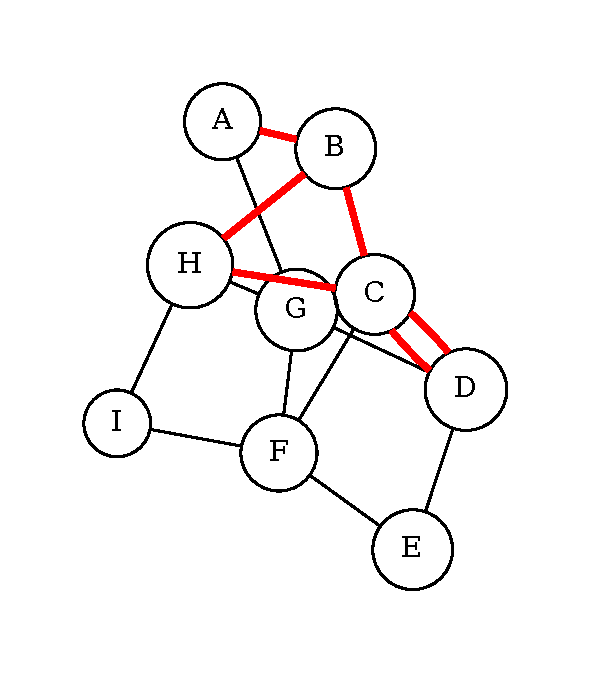
\includegraphics[width=0.5\textwidth]{Chapter2/walk.pdf}
    \end{center}
    Here, the walk shown begins at node $A$. The walk is $AB, BH, HC, CD, DC$, $CB$. The length of this walk is 6.
    \item[Trail:] A walk where all the \emph{edges} are distinct is a \textbf{trail}. The walk observed above is not a trail, since the edge $\{C, D\}$ is repeated. Thus, a variation of this as a trail might be:
    \begin{center}
        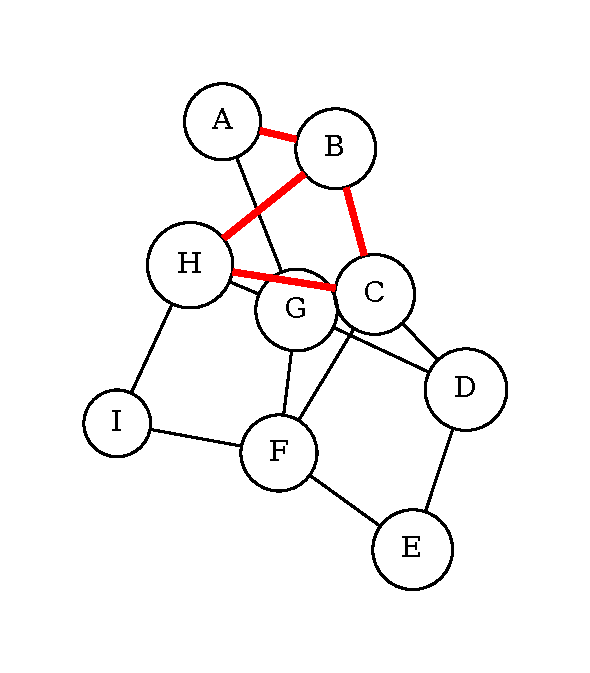
\includegraphics[width=0.5\textwidth]{Chapter2/trail.pdf}
    \end{center}
    The trail here is $AB, BH, HC, CB$.
    \item[Path:] A trail where all the \emph{vertices} are unique is called a \textbf{path}. The trail above would not be a path, as the vertex $B$ is visited twice. Here is an example of a path in $G_0$:
    \begin{center}
        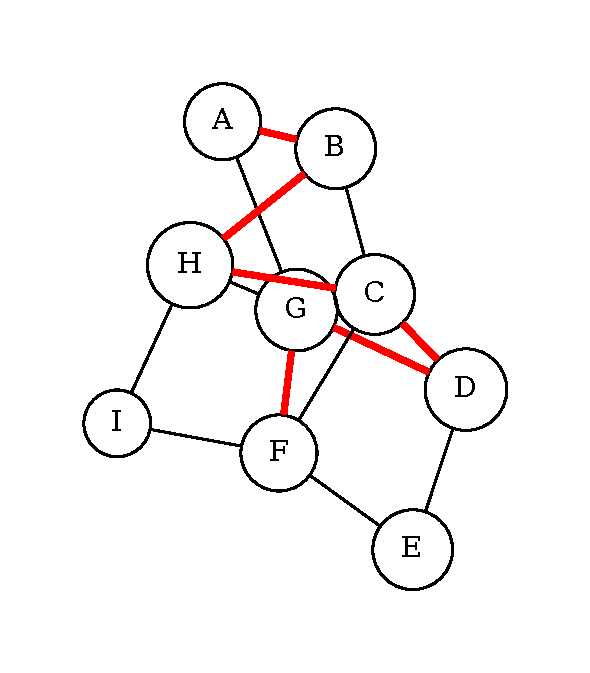
\includegraphics[width=0.5\textwidth]{Chapter2/path.pdf}
    \end{center}
    This path is $AB, BH, HC, CD, DG, GF$.
    \item[Cycle:] A \textbf{closed} path (where $v_0 = v_k$) has at least one edge, then it is a \textbf{cycle}. Here is an example of a cycle in $G_0$:
    \begin{center}
        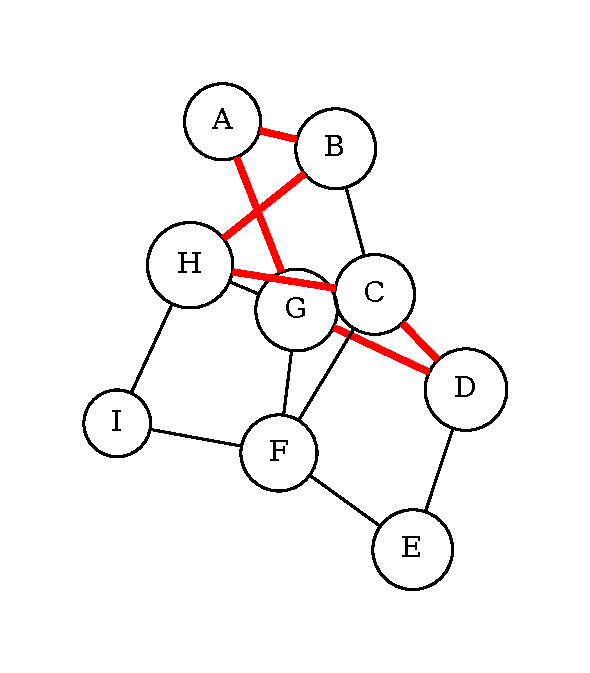
\includegraphics[width=0.5\textwidth]{Chapter2/cycle.pdf}
    \end{center}
    This cycle is $AB, BH, HC, CD, DG, GA$.     
\end{description}
\section{The Lorax}
We have the terminology we need to finally describe the subjects of this chapter: trees and forests. 
\begin{description}
    \item[Forest:] A \textbf{forest} is a graph with no cycles. It need not necessarily be connected, so long as there are no cycles. Here is an example of a forest:
    \begin{center}
        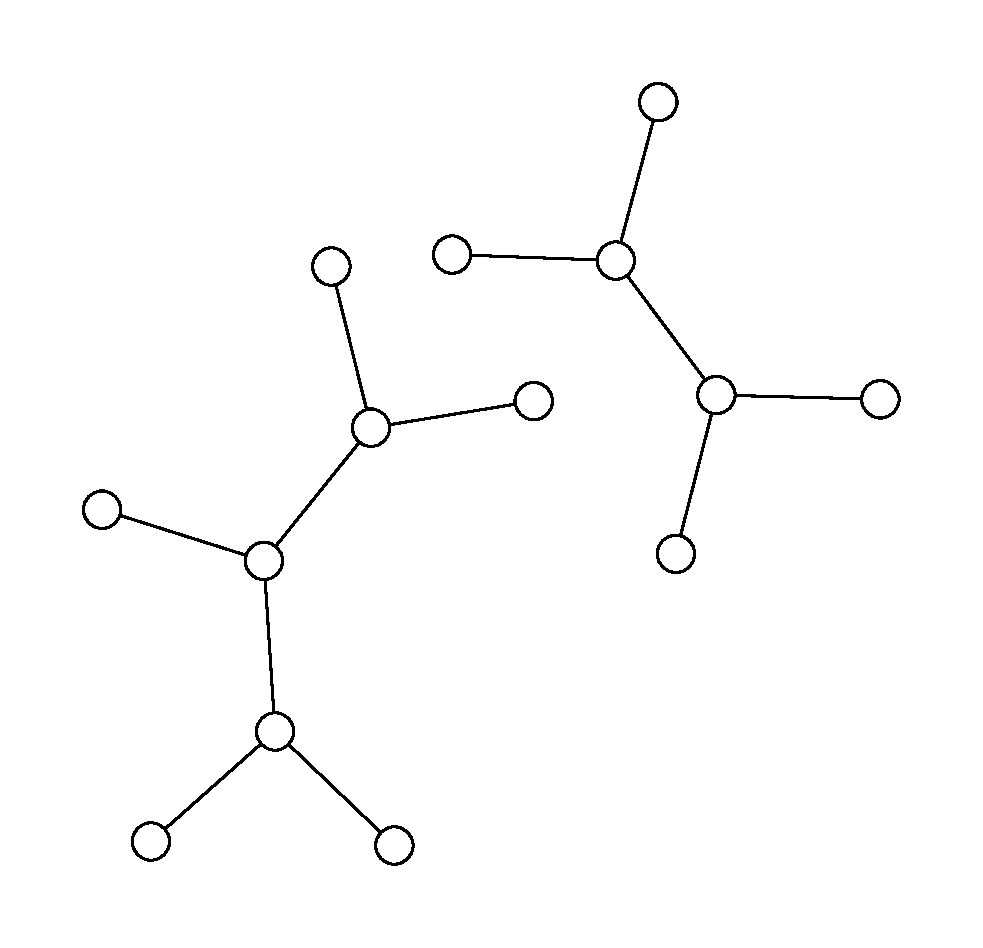
\includegraphics[width=0.5\textwidth]{Chapter2/forest.pdf}
    \end{center} 
    \item[Tree:] A \textbf{tree} is a connected forest. Here is an example of a tree:
    \begin{center}
        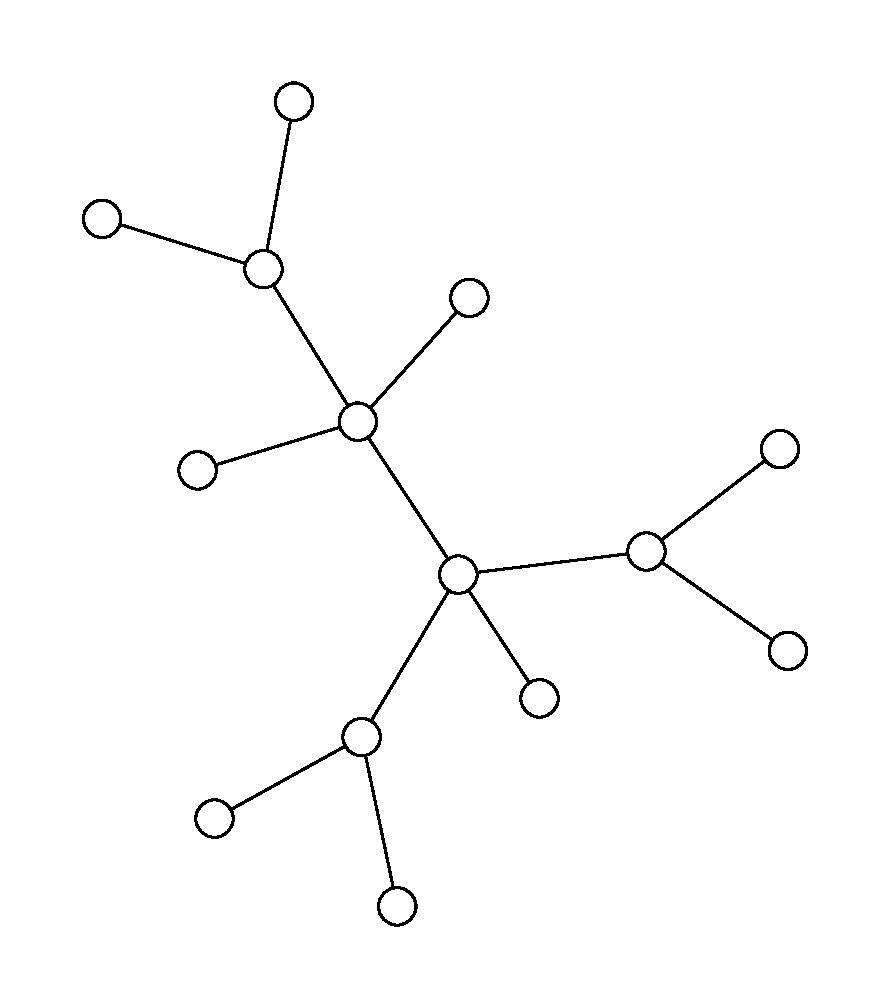
\includegraphics[width=0.5\textwidth]{Chapter2/tree.pdf}
    \end{center} 
\end{description}
Trees come in many different shapes and sizes, the count of which grows quickly as more nodes are introduces. For example, there is only one tree of one, two, and three nodes. Once we introduce a fourth node, we see that there are two distinct trees of four nodes. The more nodes we introduce, the more rapidly the count of distinct isomorphisms increases. 

\section{(Minimum) Spanning Trees}
While fundamentally trees and forests are just different kinds of graphs, they are useful tools when used in conjunction with graphs. One example of this is the \textbf{spanning tree} of a graph. The spanning tree of a graph $G$ is a tree which includes all vertices of the graph $G$. Another way to imagine this is a non-cyclic representation of $G$. On top of spanning trees, we have \textbf{minimum spanning trees} (MSTs). The MST of a graph $G$ is a spanning tree whose whose total weight is minimal compared to all spanning trees. First, let's define what a weight is.

A \textbf{weight} is a numerical value assigned to an edge. This number is representative of the total cost of traversing from one vertex to another along that particular edge - some edges may be cheaper, others may be longer. We assume that these weights are strictly non-negative (so for a weight $n, n \in \mathbb{Z}^*$). The total weight of a graph is the sum of the weights of all edges.

Again, the MST for a graph $G$ is a spanning tree with minimal weight. How do we find the minimum spanning tree for a graph? There are three popular algorithms which solve this problem: Prim's Algorithm, Kruskal's Algorithm, and Bor\r{u}vka's Algorithm.
\subsection{Prim's Algorithm}
Prim's Algorithm was originally developed by Czech mathematician Vojt\v{e}ch Jarn\'{i}k in 1930, but was later published by Robert Prim and Edsger Dijkstra in 1959\footnote{https://en.wikipedia.org/wiki/Prim's\_algorithm}. Prim's algorithm focuses on the vertices of a graph, and considers edges incident to the vertices in the MST as it grows. 

First, grab a vertex $v$ at random from a graph $G$, and initialize a tree $T$ as empty, and a set $P$ with $v$. $P$ will be our set of visited vertices, and $T$ will be the collection of edges which make the MST. Then, find the minimum weighted edge connecting a vertex in $P$ to a vertex not in $P$, and add this edge to $T$ and the vertex to $P$. Repeat until $P = V(G)$.

This algorithm is greedy - at each decision point, we follow the smallest available edge available. This results in the minimum total weight of the spanning tree, and thus gives us the MST. If we use a min-heap to store the weights of the edges of vertices in the tree, then this algorithm achieves a complexity of $O(E~log(E))$. 
\subsection{Kruskal's Algorithm}
Kruskal's Algorithm was devised the mathematician and computer scientist Joseph Kruskal in 1956\footnote{https://en.wikipedia.org/wiki/Kruskal's\_algorithm}. Unlike Prim's algorithm, which focused on the vertices of a graph, this algorithm focuses on aggregating edges in a graph until we achieve an MST. 
\subsection{Bor\r{u}vka's Algorithm}